\documentclass[a4paper,10pt,twocolumn]{article}

\usepackage{inputenc}
\usepackage{fontenc}
\usepackage{textcomp}
\usepackage{amsmath, amssymb}
\usepackage{graphicx}
\usepackage[width = 18cm,height = 22cm,columnsep = 1cm,margin = 2cm]{geometry}
\usepackage[backend=biber,style=authoryear]{biblatex}
\usepackage{aas_macros}

\bibliography{/home/riley/rproj/reports/bibliography.bib}
\graphicspath{{/home/riley/rproj/reports/images/}}

\title{Sloan Digital Sky Survey Software Development: Week 5 Progress Report}
\author{Riley Thai, Andy Casey (Supervisor)}

\newcommand{\solara}{\texttt{solara}}
\newcommand{\vaex}{\texttt{vaex}}

\begin{document}
\maketitle
\section{Aims and Objectives}
\begin{enumerate}
	\item Develop a web application for multi-dimensional exploration of SDSS-V data.
	\item Work on and contribute to the development of open-source Python libraries.
\end{enumerate}

\section{Background}
The Sloan Digital Sky Survey (SDSS) is one of the largest, longest running, and most used astronomical surveys. Started in 1998 \parencite{dr18}, the SDSS provides all-sky, multi-epoch spectroscopy using telescopes in both hemispheres, providing data used to probe the emergence of chemical elements, reveal the inner mechanisms of stars, and investigate the origin of planets. The latest generation of the survey, SDSS-V, aims to conduct the first homogeneous survey using an optical, ultra-wide integral-field spectroscopic map of the interstellar gas, pioneering spectroscopic monitoring and revealing changes on both short and vast timescales \parencite{SDSS2017}. SDSS data over all survey phases has been cited more than 650,000 over 111,000 refereed papers \parencite{dr18}.

The SDSS has previously offered a simple web application for end users to access, explore, and investigate spectra and other data. However, the fifth generation of the survey now offers a large catalog of stars with complete stellar labels. With a larger set of spectral types explored \parencite{apogee2017}, and an even larger set of stellar labels (Casey et al., in prep), there is a need for a new tool which provides powerful exploration and visualization of large and vast datasets.

\section{\texttt{specutils} Development}
To be familiar with the variety of SDSS-V datatypes, I first began this project by developing loaders for the new SDSS-V datatypes. Within the Python library \texttt{specutils}, which provides tools to the \texttt{astropy} library for handling spectral data, there are a class of objects used for representing spectra, named  \texttt{Spectrum1D} and \texttt{SpectrumList}. I created default loading functions for both the new and updated datatypes within the SDSS-V dataset. Built in as the sub-method to each \texttt{Spectrum} class, by specifying a filepath, a user can read a single or all spectrum from a given SDSS data file.

Most importantly, the default loader allows for any third party which use the \texttt{specutils Spectrum} objects to load the new SDSS-V datatypes, such as the Jdaviz spectrum viewer, shown in Figure \ref{fig:jdaviz}.

\begin{figure}[htpb]
	\centering
	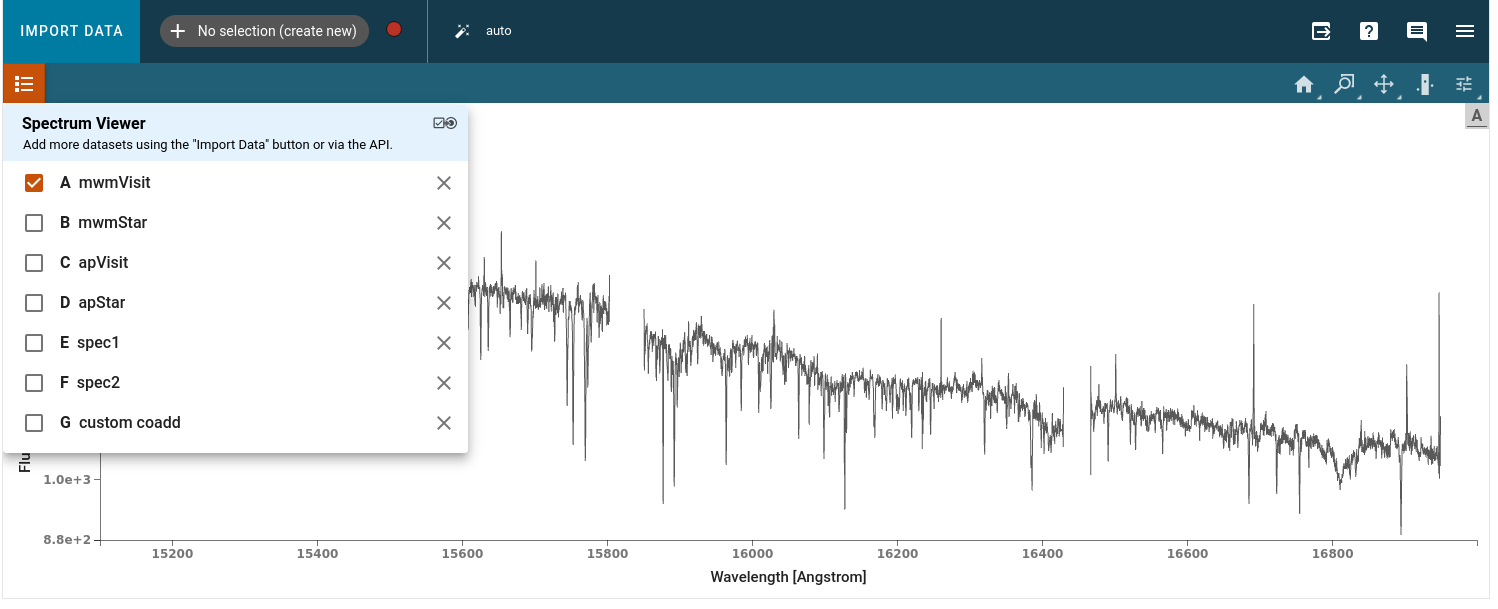
\includegraphics[width=\columnwidth]{jdaviz}
	\caption{Spectrum data from a BOSS spectrograph, as shown within jdaviz SpectrumViewer.}
	\label{fig:jdaviz}
\end{figure}

\section{Plotting Dashboard Development}
After completing the new loaders, I began work on the parameter dashboard. The dashboard leverages the out-of-memory dataframes and high-speed aggregations of \vaex, and combines them with the React-like framework in Python, \solara, to deliver an intuitive, but powerful visualization tool for the large SDSS datasets. The data is read out of memory from an Apache Arrow format, dramatically reducing system overhead, both client and server-side.

Currently, the dashboard can be used to investigate any uploaded file, or a small subset of SDSS-V data. The main method of interaction is through a sidebar on the left, which allows the user to change plotting parameters, such as the x-y scale, columns, number of bins, and type of statistic to overplot with.

\begin{figure}[htpb]
	\centering
	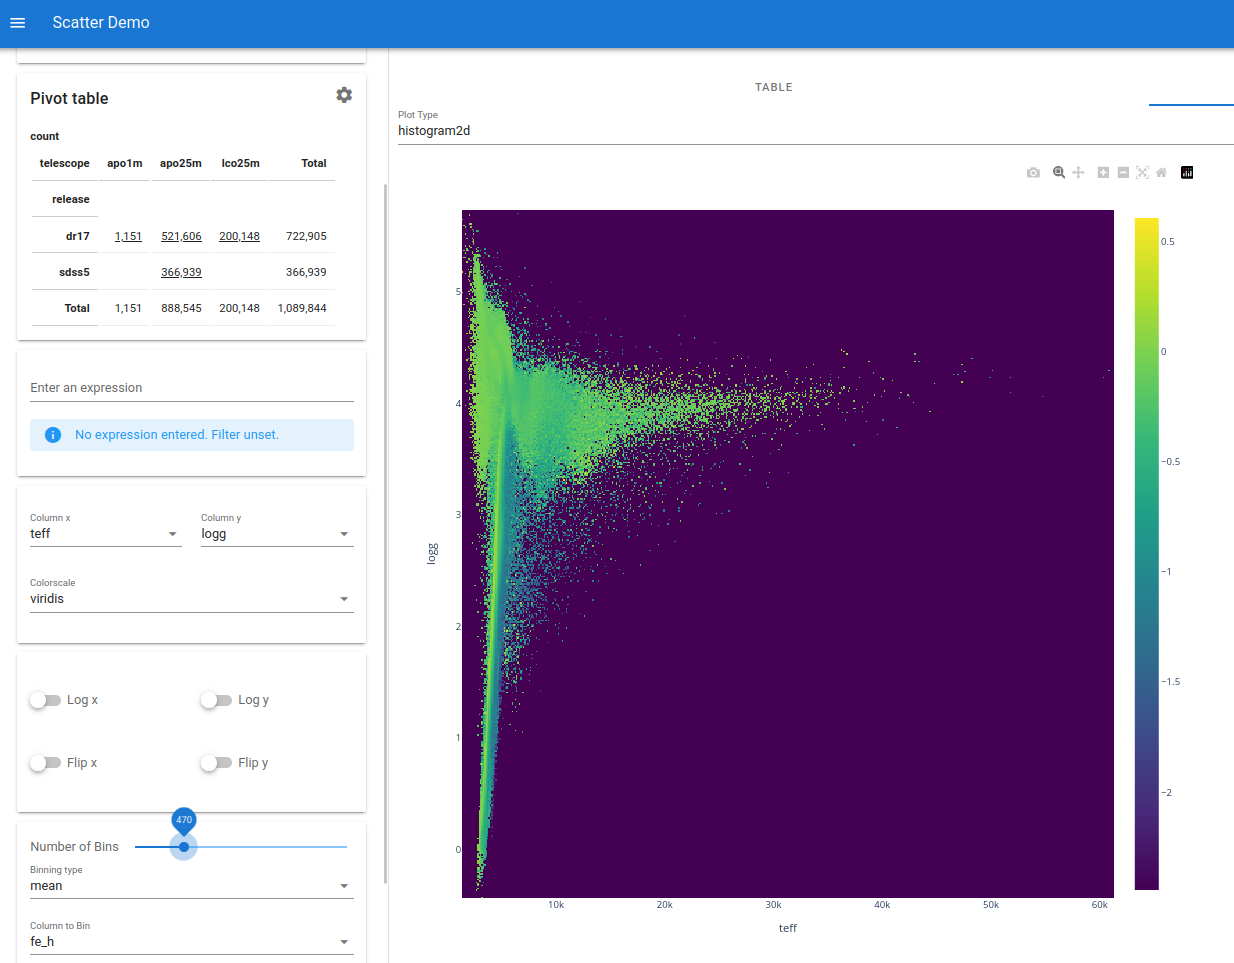
\includegraphics[width=\columnwidth]{2d}
	\caption{A display showing the histogram2d plotting mode with sample data. The data is read from a \texttt{parquet} file, which reduces the memory overhead of the application. It is then delivered to the application by a \vaex dataframe, and plotted with \texttt{Plotly} and shown in a \solara application (the dashboard).}
	\label{fig:2d}
\end{figure}

The dashboard has 3 modes: histogram, in one and two dimensions, and a scatter plot. These were likely to be the most useful for data exploration, so they were implemented first.

The dashboard's \texttt{histogram2d} mode heavily utilizes \vaex's aggregated statistics over grids, which allows for complex multi-dimensional plotting, without suffering from the pitfalls of scatter plots, such as overplotting the dataset or underrepresenting through downsampling. This view is shown in Figure \ref{fig:2d}.

The most advanced feature implemented so far is the expression editor, which allows the user to leverage vaex's high-speed computations to filter the dataset. This can be combined with other filtering methods, such as a pivot table and/or selection, to directly select a complex subset of data. This functionality is shown in Figure \ref{fig:expression}.

\begin{figure*}[htpb]
	\centering
	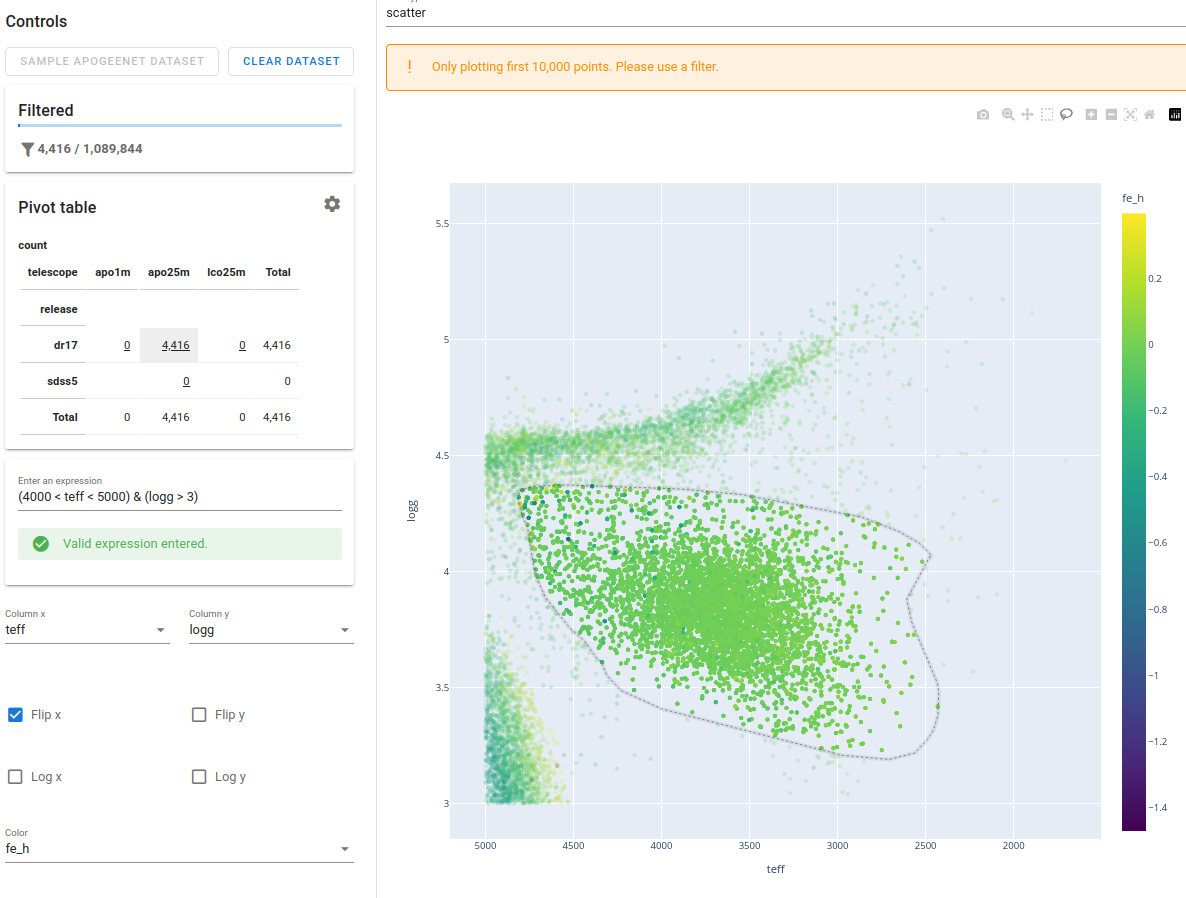
\includegraphics[width=0.85\textwidth]{expression}
	\caption{A showcase of the full cross-filtering functionality within the scatter plot. A filter is applied by an expression, then a subset is chosen using the pivot table (left). Finally a subset of the data can be selected within the scatter plot via the lasoo tool.}
	\label{fig:expression}
\end{figure*}

\section{Difficulties encountered}
\begin{enumerate}
	\item \textbf{\texttt{vaex} and \texttt{solara} documentation is often incomplete.}
	      \begin{itemize}
		      \item Throughout development, I found several functions within the source code that were not apparent on the API documentation.
		      \item This is common throughout open-source development, due to its decentralized nature, but I will also endeavour to ensure I properly document my work.
	      \end{itemize}
	\item \textbf{Error messages from \solara are obtuse (no traceback to soure code).}
	      \begin{itemize}
		      \item When testing the web app, any bugs which arise often don't provide clear tracebacks, often stopping at one function, or only returning that there was an error during rendering.
		      \item This is due to the way \solara runs the web application on its own server, which prevents these from appearing.
		      \item This has made it more difficult, but not impossible, to track down bugs, as I can't use debuggers or other tools directly.
	      \end{itemize}
\end{enumerate}
\section{Future plans}
\begin{enumerate}
	\item \textbf{Expand cross-filtering functionality.}
	      \begin{enumerate}
		      \item We can expand the cross-filtering functionality to further leverage \vaex functionality.
		      \item Possible expansions include:
		            \begin{itemize}
			            \item using the groupby object, similar to how it is implemented in \texttt{pandas}.
			            \item allowing for the selection of a specific bin within the histogram2d view.
			            \item expanding to have different subsets saved for the user to use and explore individually, rather than across the entire dashboard.
		            \end{itemize}
	      \end{enumerate}
	\item \textbf{Implement the webapp within the proprietary backend.}
	      \begin{enumerate}
		      \item SDSS uses a backend derivative based on FastAPI. Currently, the webapp we've developed works on Starlette, but hasn't been implemented in the proprietary backend yet.
		      \item This is due to a few bugs during startup of the development Docker setup which we still need to resolve, which will help other members of the collaboration to test it as well.
	      \end{enumerate}
\end{enumerate}
\printbibliography
\end{document}


